\documentclass[12pt,twoside]{article}

\newcommand{\reporttitle}{Mathematics for Machine Learning}
\newcommand{\reportauthor}{Alexander Gaskell}
\newcommand{\reporttype}{Coursework}
\newcommand{\cid}{01813313}

% include files that load packages and define macros
%%%%%%%%%%%%%%%%%%%%%%%%%%%%%%%%%%%%%%%%%
% University Assignment Title Page 
% LaTeX Template
% Version 1.0 (27/12/12)
%
% This template has been downloaded from:
% http://www.LaTeXTemplates.com
%
% Original author:
% WikiBooks (http://en.wikibooks.org/wiki/LaTeX/Title_Creation)
%
% License:
% CC BY-NC-SA 3.0 (http://creativecommons.org/licenses/by-nc-sa/3.0/)
% 
% Instructions for using this template:
% This title page is capable of being compiled as is. This is not useful for 
% including it in another document. To do this, you have two options: 
%
% 1) Copy/paste everything between \begin{document} and \end{document} 
% starting at \begin{titlepage} and paste this into another LaTeX file where you 
% want your title page.
% OR
% 2) Remove everything outside the \begin{titlepage} and \end{titlepage} and 
% move this file to the same directory as the LaTeX file you wish to add it to. 
% Then add \input{./title_page_1.tex} to your LaTeX file where you want your
% title page.
%
%----------------------------------------------------------------------------------------
%	PACKAGES AND OTHER DOCUMENT CONFIGURATIONS
%----------------------------------------------------------------------------------------
\usepackage{ifxetex}
\usepackage{textpos}
\usepackage{natbib}
\usepackage{kpfonts}
\usepackage[a4paper,hmargin=2.8cm,vmargin=2.0cm,includeheadfoot]{geometry}
\usepackage{ifxetex}
\usepackage{stackengine}
\usepackage{tabularx,longtable,multirow,subfigure,caption}%hangcaption
\usepackage{fncylab} %formatting of labels
\usepackage{fancyhdr}
\usepackage{color}
\usepackage[tight,ugly]{units}
\usepackage{url}
\usepackage{float}
\usepackage[english]{babel}
\usepackage{amsmath}
\usepackage{graphicx}
\usepackage[colorinlistoftodos]{todonotes}
\usepackage{dsfont}
\usepackage{epstopdf} % automatically replace .eps with .pdf in graphics
\usepackage{natbib}
\usepackage{backref}
\usepackage{array}
\usepackage{latexsym}
\usepackage{etoolbox}

\usepackage{enumerate} % for numbering with [a)] format 



\ifxetex
\usepackage{fontspec}
\setmainfont[Scale=.8]{OpenDyslexic-Regular}
\else
\usepackage[pdftex,pagebackref,hypertexnames=false,colorlinks]{hyperref} % provide links in pdf
\hypersetup{pdftitle={},
  pdfsubject={}, 
  pdfauthor={\reportauthor},
  pdfkeywords={}, 
  pdfstartview=FitH,
  pdfpagemode={UseOutlines},% None, FullScreen, UseOutlines
  bookmarksnumbered=true, bookmarksopen=true, colorlinks,
    citecolor=black,%
    filecolor=black,%
    linkcolor=black,%
    urlcolor=black}
\usepackage[all]{hypcap}
\fi

\usepackage{tcolorbox}

% various theorems
\usepackage{ntheorem}
\theoremstyle{break}
\newtheorem{lemma}{Lemma}
\newtheorem{theorem}{Theorem}
\newtheorem{remark}{Remark}
\newtheorem{definition}{Definition}
\newtheorem{proof}{Proof}

% example-environment
\newenvironment{example}[1][]
{ 
\vspace{4mm}
\noindent\makebox[\linewidth]{\rule{\hsize}{1.5pt}}
\textbf{Example #1}\\
}
{ 
\noindent\newline\makebox[\linewidth]{\rule{\hsize}{1.0pt}}
}



%\renewcommand{\rmdefault}{pplx} % Palatino
% \renewcommand{\rmdefault}{put} % Utopia

\ifxetex
\else
\renewcommand*{\rmdefault}{bch} % Charter
\renewcommand*{\ttdefault}{cmtt} % Computer Modern Typewriter
%\renewcommand*{\rmdefault}{phv} % Helvetica
%\renewcommand*{\rmdefault}{iwona} % Avant Garde
\fi

\setlength{\parindent}{0em}  % indentation of paragraph

\setlength{\headheight}{14.5pt}
\pagestyle{fancy}
\fancyfoot[ER,OL]{\thepage}%Page no. in the left on
                                %odd pages and on right on even pages
\fancyfoot[OC,EC]{\sffamily }
\renewcommand{\headrulewidth}{0.1pt}
\renewcommand{\footrulewidth}{0.1pt}
\captionsetup{margin=10pt,font=small,labelfont=bf}


%--- chapter heading

\def\@makechapterhead#1{%
  \vspace*{10\p@}%
  {\parindent \z@ \raggedright %\sffamily
        %{\Large \MakeUppercase{\@chapapp} \space \thechapter}
        %\\
        %\hrulefill
        %\par\nobreak
        %\vskip 10\p@
    \interlinepenalty\@M
    \Huge \bfseries 
    \thechapter \space\space #1\par\nobreak
    \vskip 30\p@
  }}

%---chapter heading for \chapter*  
\def\@makeschapterhead#1{%
  \vspace*{10\p@}%
  {\parindent \z@ \raggedright
    \sffamily
    \interlinepenalty\@M
    \Huge \bfseries  
    #1\par\nobreak
    \vskip 30\p@
  }}
  



% %%%%%%%%%%%%% boxit
\def\Beginboxit
   {\par
    \vbox\bgroup
	   \hrule
	   \hbox\bgroup
		  \vrule \kern1.2pt %
		  \vbox\bgroup\kern1.2pt
   }

\def\Endboxit{%
			      \kern1.2pt
		       \egroup
		  \kern1.2pt\vrule
		\egroup
	   \hrule
	 \egroup
   }	

\newenvironment{boxit}{\Beginboxit}{\Endboxit}
\newenvironment{boxit*}{\Beginboxit\hbox to\hsize{}}{\Endboxit}



\allowdisplaybreaks

\makeatletter
\newcounter{elimination@steps}
\newcolumntype{R}[1]{>{\raggedleft\arraybackslash$}p{#1}<{$}}
\def\elimination@num@rights{}
\def\elimination@num@variables{}
\def\elimination@col@width{}
\newenvironment{elimination}[4][0]
{
    \setcounter{elimination@steps}{0}
    \def\elimination@num@rights{#1}
    \def\elimination@num@variables{#2}
    \def\elimination@col@width{#3}
    \renewcommand{\arraystretch}{#4}
    \start@align\@ne\st@rredtrue\m@ne
}
{
    \endalign
    \ignorespacesafterend
}
\newcommand{\eliminationstep}[2]
{
    \ifnum\value{elimination@steps}>0\leadsto\quad\fi
    \left[
        \ifnum\elimination@num@rights>0
            \begin{array}
            {@{}*{\elimination@num@variables}{R{\elimination@col@width}}
            |@{}*{\elimination@num@rights}{R{\elimination@col@width}}}
        \else
            \begin{array}
            {@{}*{\elimination@num@variables}{R{\elimination@col@width}}}
        \fi
            #1
        \end{array}
    \right]
    & 
    \begin{array}{l}
        #2
    \end{array}
    &%                                    moved second & here
    \addtocounter{elimination@steps}{1}
}
\makeatother

%% Fast macro for column vectors
\makeatletter  
\def\colvec#1{\expandafter\colvec@i#1,,,,,,,,,\@nil}
\def\colvec@i#1,#2,#3,#4,#5,#6,#7,#8,#9\@nil{% 
  \ifx$#2$ \begin{bmatrix}#1\end{bmatrix} \else
    \ifx$#3$ \begin{bmatrix}#1\\#2\end{bmatrix} \else
      \ifx$#4$ \begin{bmatrix}#1\\#2\\#3\end{bmatrix}\else
        \ifx$#5$ \begin{bmatrix}#1\\#2\\#3\\#4\end{bmatrix}\else
          \ifx$#6$ \begin{bmatrix}#1\\#2\\#3\\#4\\#5\end{bmatrix}\else
            \ifx$#7$ \begin{bmatrix}#1\\#2\\#3\\#4\\#5\\#6\end{bmatrix}\else
              \ifx$#8$ \begin{bmatrix}#1\\#2\\#3\\#4\\#5\\#6\\#7\end{bmatrix}\else
                 \PackageError{Column Vector}{The vector you tried to write is too big, use bmatrix instead}{Try using the bmatrix environment}
              \fi
            \fi
          \fi
        \fi
      \fi
    \fi
  \fi 
}  
\makeatother

\robustify{\colvec}

%%% Local Variables: 
%%% mode: latex
%%% TeX-master: "notes"
%%% End: 
 % various packages needed for maths etc.
% quick way of adding a figure
\newcommand{\fig}[3]{
 \begin{center}
 \scalebox{#3}{\includegraphics[#2]{#1}}
 \end{center}
}

%\newcommand*{\point}[1]{\vec{\mkern0mu#1}}
\newcommand{\ci}[0]{\perp\!\!\!\!\!\perp} % conditional independence
\newcommand{\point}[1]{{#1}} % points 
\renewcommand{\vec}[1]{{\boldsymbol{{#1}}}} % vector
\newcommand{\mat}[1]{{\boldsymbol{{#1}}}} % matrix
\newcommand{\R}[0]{\mathds{R}} % real numbers
\newcommand{\Z}[0]{\mathds{Z}} % integers
\newcommand{\N}[0]{\mathds{N}} % natural numbers
\newcommand{\nat}[0]{\mathds{N}} % natural numbers
\newcommand{\Q}[0]{\mathds{Q}} % rational numbers
\ifxetex
\newcommand{\C}[0]{\mathds{C}} % complex numbers
\else
\newcommand{\C}[0]{\mathds{C}} % complex numbers
\fi
\newcommand{\tr}[0]{\text{tr}} % trace
\renewcommand{\d}[0]{\mathrm{d}} % total derivative
\newcommand{\inv}{^{-1}} % inverse
\newcommand{\id}{\mathrm{id}} % identity mapping
\renewcommand{\dim}{\mathrm{dim}} % dimension
\newcommand{\rank}[0]{\mathrm{rk}} % rank
\newcommand{\determ}[1]{\mathrm{det}(#1)} % determinant
\newcommand{\scp}[2]{\langle #1 , #2 \rangle}
\newcommand{\kernel}[0]{\mathrm{ker}} % kernel/nullspace
\newcommand{\img}[0]{\mathrm{Im}} % image
\newcommand{\idx}[1]{{(#1)}}
\DeclareMathOperator*{\diag}{diag}
\newcommand{\E}{\mathds{E}} % expectation
\newcommand{\var}{\mathds{V}} % variance
\newcommand{\gauss}[2]{\mathcal{N}\big(#1,\,#2\big)} % gaussian distribution N(.,.)
\newcommand{\gaussx}[3]{\mathcal{N}\big(#1\,|\,#2,\,#3\big)} % gaussian distribution N(.|.,.)
\newcommand{\gaussBig}[2]{\mathcal{N}\left(#1,\,#2\right)} % see above, but with brackets that adjust to the height of the arguments
\newcommand{\gaussxBig}[3]{\mathcal{N}\left(#1\,|\,#2,\,#3\right)} % see above, but with brackets that adjust to the height of the arguments
\DeclareMathOperator{\cov}{Cov} % covariance (matrix) 
\ifxetex
\renewcommand{\T}[0]{^\top} % transpose
\else
\newcommand{\T}[0]{^\top}
\fi
% matrix determinant
\newcommand{\matdet}[1]{
\left|
\begin{matrix}
#1
\end{matrix}
\right|
}



%%% various color definitions
\definecolor{darkgreen}{rgb}{0,0.6,0}

\newcommand{\blue}[1]{{\color{blue}#1}}
\newcommand{\red}[1]{{\color{red}#1}}
\newcommand{\green}[1]{{\color{darkgreen}#1}}
\newcommand{\orange}[1]{{\color{orange}#1}}
\newcommand{\magenta}[1]{{\color{magenta}#1}}
\newcommand{\cyan}[1]{{\color{cyan}#1}}


% redefine emph
\renewcommand{\emph}[1]{\blue{\bf{#1}}}

% place a colored box around a character
\gdef\colchar#1#2{%
  \tikz[baseline]{%
  \node[anchor=base,inner sep=2pt,outer sep=0pt,fill = #2!20] {#1};
    }%
}%
 % short-hand notation and macros

% additional packages for this report
\usepackage{tikz}
\usetikzlibrary{bayesnet}
\usepackage{enumitem}

%%%%%%%%%%%%%%%%%%%%%%%%%%%%

\begin{document}
% front page
% Last modification: 2016-09-29 (Marc Deisenroth)
\begin{titlepage}

\newcommand{\HRule}{\rule{\linewidth}{0.5mm}} % Defines a new command for the horizontal lines, change thickness here


%----------------------------------------------------------------------------------------
%	LOGO SECTION
%----------------------------------------------------------------------------------------


\includegraphics[width = 4cm]{./figures/imperial}\\[0.5cm] 

\begin{center} % Center remainder of the page

%----------------------------------------------------------------------------------------
%	HEADING SECTIONS
%----------------------------------------------------------------------------------------
\textsc{\LARGE \reporttype}\\[1.5cm] 
\textsc{\Large Imperial College London}\\[0.5cm] 
\textsc{\large Department of Computing}\\[0.5cm] 
%----------------------------------------------------------------------------------------
%	TITLE SECTION
%----------------------------------------------------------------------------------------

\HRule \\[0.4cm]
{ \huge \bfseries \reporttitle}\\ % Title of your document
\HRule \\[1.5cm]
\end{center}
%----------------------------------------------------------------------------------------
%	AUTHOR SECTION
%----------------------------------------------------------------------------------------

%\begin{minipage}{0.4\hsize}
\begin{flushleft} \large
\textit{Author:}\\
\reportauthor~(CID: \cid) \\% Your name 
\textit{Email:} \\
\reportemail
\end{flushleft}
\vspace{2cm}
\makeatletter
Date: \@date 

\vfill % Fill the rest of the page with whitespace



\makeatother


\end{titlepage}




%%%%%%%%%%%%%%%%%%%%%%%%%%%% Main document
\section{Statistics and Probabilities}
\subsection{}
\textbf{[8 marks]Compute the sample mean and the sample covariance matrix of the following dataset (use 1/N for the covariance matrix). Describe the computations you used to get to the answer.}
\begin{align}
D = [\colvec{1,2,3},\, \colvec{-1,0,0},\, \colvec{-4,4,2}]
= [\vec x_{1},\vec x_{2},\vec x_{3}]
\end{align}
Sample mean is calculated as follows:    
\begin{equation}
    \overline{\vec x} = \frac{1}{N}\sum^{N}_{n=1}\vec x_{n}, \quad \vec x \in \mathbb{R}^3
\end{equation}
Hence to find the mean vector we sum horizontally for each row and divide by the number of samples (in this instance, 3). For example, to calculate $\overline{x_1}$, the calculation is $(1+(-1)+(-4))/3 = -4/3$. 
Thus the sample mean is:
\begin{align}\overline{\vec x} = \begin{bmatrix} -4/3 \\ 2 \\ 5/3 \end{bmatrix}\end{align}
Sample covariance can be found as follows:
\begin{equation}
    \operatorname{Cov}[D] = \operatorname{E}[(\vec x - \overline{\vec x})^2]=\frac{1}{N}\sum^{N}_{n=1}(\vec x_n-\overline{\vec x})(\vec x_n-\overline{\vec x})\T
\end{equation}
This shows that the covariance is found by taking the mean of $N$ outer products, where each outer product is composed of a single de-meaned sample multiplied by its transpose. So $\operatorname{Cov}[D]$ is calculated by the following:
\begin{align}
    \operatorname{Cov}[D] &= \frac{1}{3} 
        \begin{pmatrix}
            \begin{pmatrix} \vec x_1 - \overline{\vec x} \end{pmatrix} 
            \begin{pmatrix} \vec x_1\T - \overline{\vec x}\T \end{pmatrix} +
            \begin{pmatrix} \vec x_2 - \overline{\vec x} \end{pmatrix}
            \begin{pmatrix} \vec x_2\T - \overline{\vec x}\T \end{pmatrix} +
            \begin{pmatrix} \vec x_3 - \overline{\vec x} \end{pmatrix}
            \begin{pmatrix} \vec x_3\T - \overline{\vec x}\T \end{pmatrix}
        \end{pmatrix} \\
        & = \frac{1}{9}
        \left[
        \begin{array}{ccc}
            38  & -18 &  5\\
            -18  & 24  & 12 \\
            5  & 12 & 14 
        \end{array}
        \right]
        =
        \left[
        \begin{array}{ccc}
            4.2  & -2.0 &  0.6\\
            -2.0  & 2.7  & 1.3 \\
            0.6  & 1.3 & 1.6 
        \end{array}
        \right]
\end{align}
\pagebreak{}

\subsection{}
\textbf{[9 marks]Generate two datasets $\{(x_1,x_2)_n\}$ of 100 data points each. The datasets have mean:
$\mu = \colvec{-1, 1}$
and marginal variances $\sigma_1^2 = 2, \sigma^2_2 = 0.5$. Ensure that the shape of the datasets you generate is different. Visualize the two datasets and explain how you generated them so that their shapes are different.}
\smallbreak
Given the above specifications on mean vector and marginal covariances, a sample can be generated from drawing from the following Gaussian distribution:
\begin{equation}
    p(\vec x|\vec \mu,\Sigma) = \mathcal{N}(\colvec{-1,1}, \begin{bmatrix} 2 & \sigma^2_{x_1,x_2} \\ \sigma^2_{x_2,x_1} & 0.5 \end{bmatrix})
\end{equation}
Where $\sigma^2_{x_1,x_2}$ and $\sigma^2_{x_2,x_1}$ can be modified to change the shape of the distribution (provided the covariance matrix is positive semi-definite). 
The sample plotted in figure \ref{G1} is drawn from the following distribution:
\begin{equation}
    p(\vec x|\vec \mu,\Sigma) = \mathcal{N}(\colvec{-1,1}, \begin{bmatrix} 2 & 0 \\ 0 & 0.5 \end{bmatrix}) = G_1
\end{equation}
This can be contrasted with figure \ref{G2}, drawn from the distribution:
\begin{equation}
    p(\vec x|\vec \mu,\Sigma) = \mathcal{N}(\colvec{-1,1}, \begin{bmatrix} 2 & -0.5 \\ -0.5 & 0.5 \end{bmatrix}) = G_2
\end{equation}
Both of these samples are plotted below. For figure \ref{G1} below, the 100 samples drawn from $G_1$ appear as blue dots on the right-hand plot. They have been plotted on top of the contour plot of $G_1$, and alongside the mesh plot of $G_1$, both visualizing the probability density of $G_1$. $G_2$ has likewise been plotted below in figure \ref{G2}.
\smallbreak
Inspection of of the contour plots and sample plots in figures \ref{G1} and \ref{G2} show that setting the cross covariance terms to $-0.5$ has the effect of tilting the axis of the distribution (or "squish" the distribution along the axis $x_1 = 2x_2$). This is because the cross covariance terms dictate the correlation between $x_1$ and $x_2$, so setting this to $-0.5$ creates a negative relationship between $x_1$ and $x_2$ in $G_2$.
\pagebreak

\begin{figure}[h]
\centering % this centers the figure
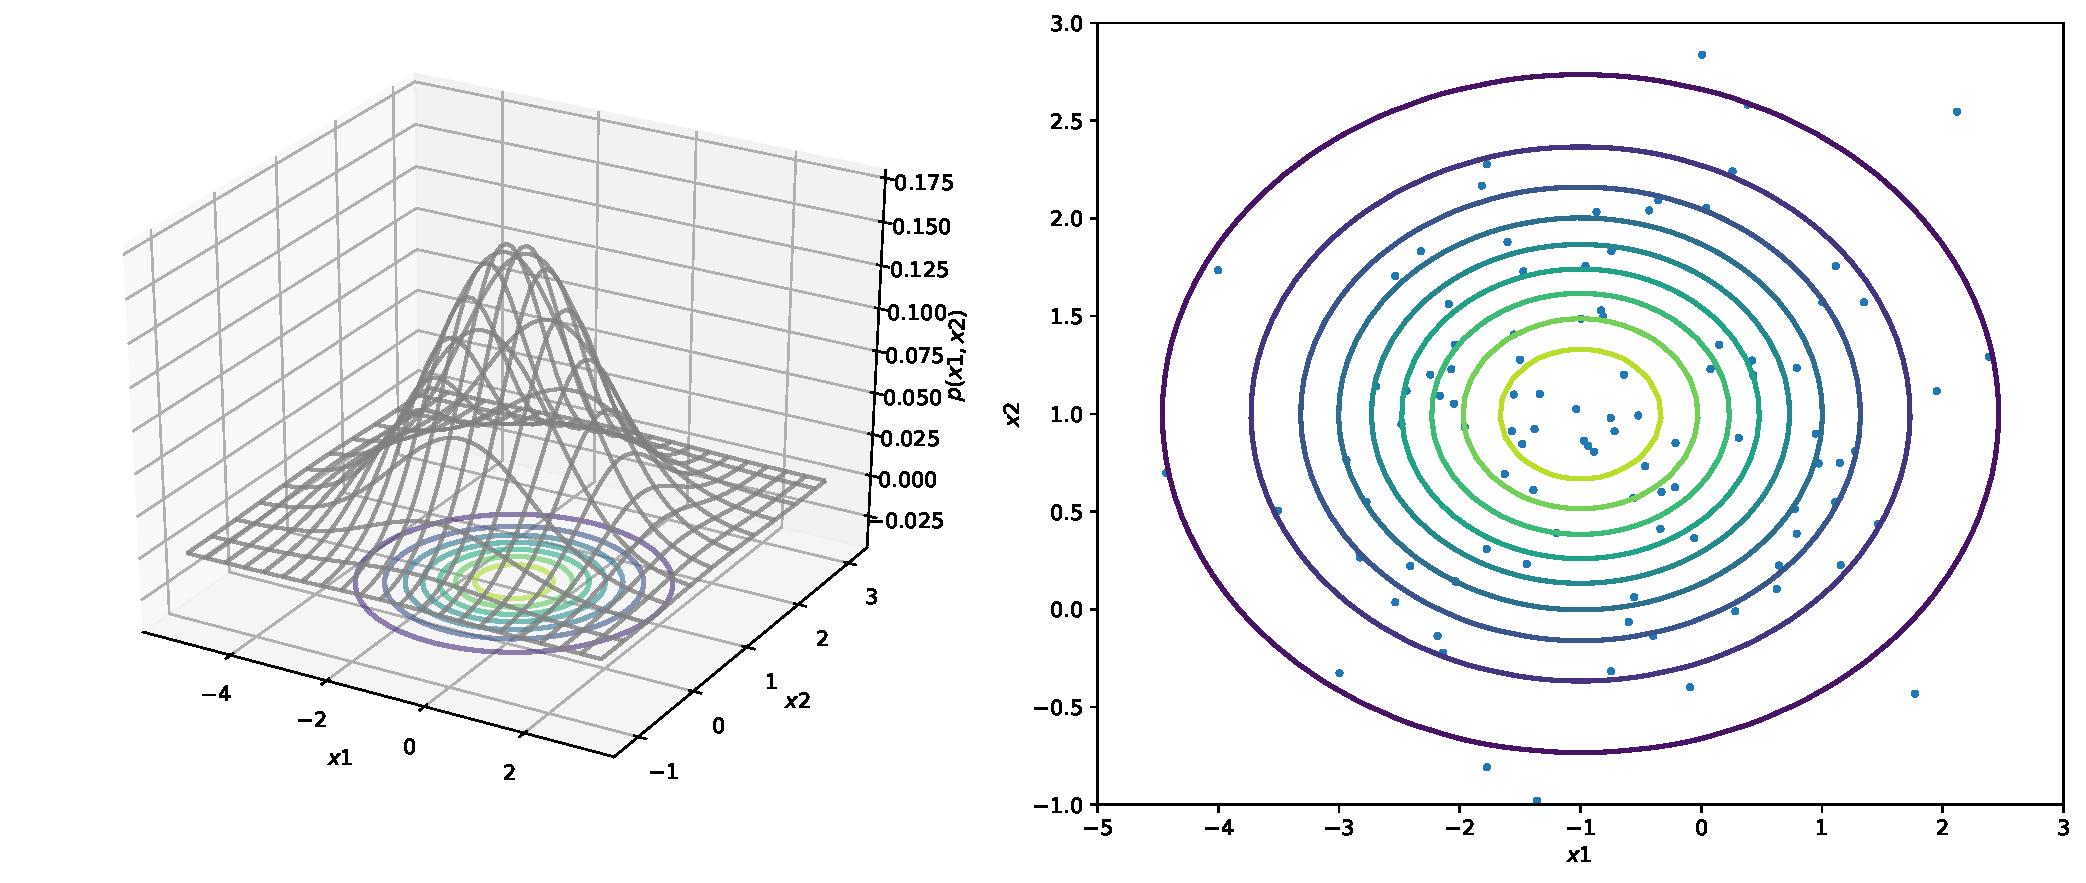
\includegraphics[width = 1\hsize]{./figures/gaussian3da.pdf} % this includes the figure and %specifies that it should span 0.7 times the horizontal size of the page
\caption{Pdf and contour plots  for $G_1$ where $\sigma^2_{x_1,x_2} = \sigma^2_{x_2,x_1} = 0$ } % caption of the figure
\label{G1}
\end{figure}

\begin{figure}[h]
\centering % this centers the figure
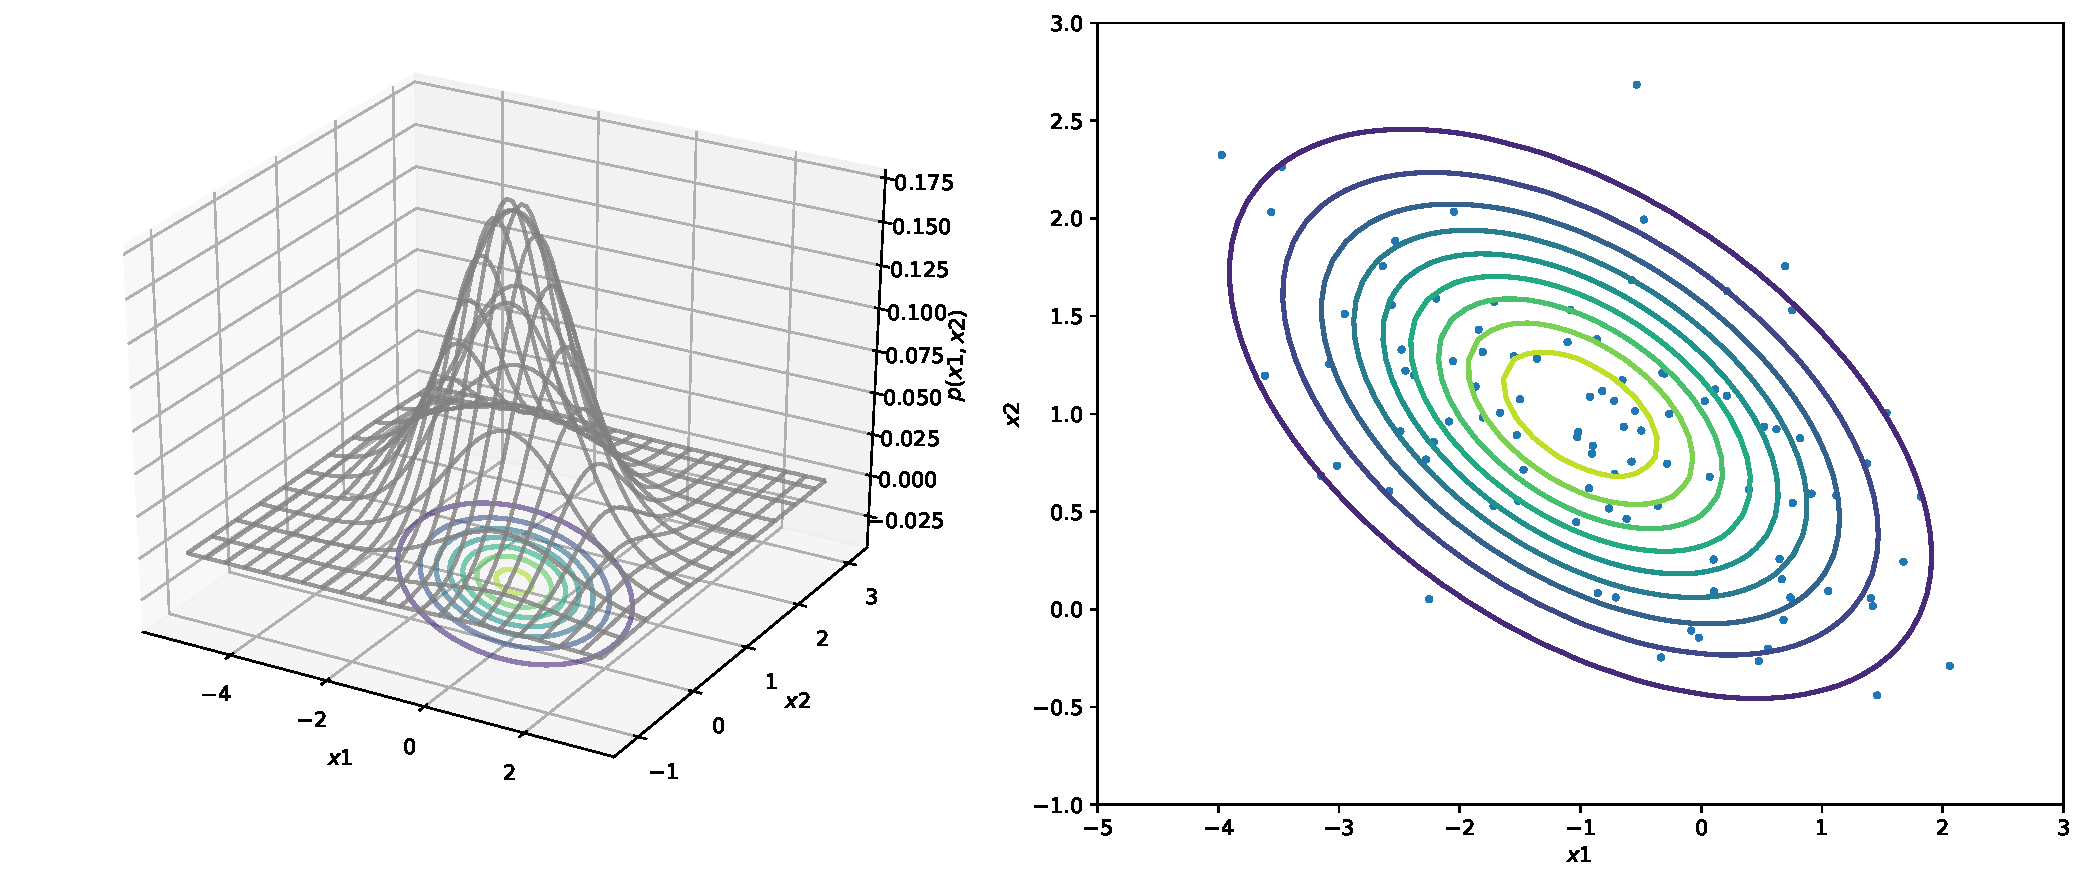
\includegraphics[width = 1\hsize]{./figures/gaussian3db.pdf} % this includes the figure and %specifies that it should span 0.7 times the horizontal size of the page
\caption{Pdf and contour plots  for $G_2$ where $\sigma^2_{x_1,x_2} = \sigma^2_{x_2,x_1} = -0.5$ } % caption of the figure
\label{G2}
\end{figure}


\subsection{}
\textbf{[27 marks] Nora and Noah spent the summer on writing a computer program that solves AI. However, they encounter the problem that their code seems to be failing randomly when compiling. Nora and Noah want to estimate the probability of successful compilation using a probabilistic model. They assume that when compiling the 
code $N$ times (without any changes to the code) gives i.i.d. results. Furthermore, the probability of success can be described by a Bernoulli distribution with an unknown parameter $\mu$. As good Bayesians, they place a conjugate Beta prior on this unknown parameter, where the parameters of this beta prior are $\alpha = 2, \beta = 2$ . They have now run $N = 20$ experiments, and 6 of them successfully compiles, and 14 failed.
\begin{itemize}
    \item Compute the posterior distribution on $\mu$ (derive your result) and plot it.
\end{itemize}}

The prior follows a $\operatorname{Beta(2,2)}$ distribution:
\begin{align}
    p(\mu|\alpha,\beta) = p(\mu|2,2) =\frac{\Gamma(2+2)}{\Gamma(2)\Gamma(2)}\mu^{2-1}(1-\mu)^{2-1} = 6\mu(1-\mu)
\end{align}
The likelihood can be modelled as a Binomial distribution given that it is multiple trials of a Bernoulli random variable. Hence the likelihood is:
\begin{align}
    p(x|N,\mu) = p(6|20,\mu) = \begin{pmatrix}20 \\6\end{pmatrix}\mu^6(1-\mu)^{14}
\end{align}
By Bayes' theorem, we can compute the posterior as being proportional to the prior and the likelihood:
\begin{align}
    posterior = \frac{prior*likelihood}{evidence} \propto prior*likelihood
\end{align}
Hence the posterior can be drived as follows:
\begin{align}
\label{posterior}
    posterior \propto 6\mu(1-\mu)*\begin{pmatrix}20 \\6\end{pmatrix}\mu^6(1-\mu)^{14} = 6\begin{pmatrix}20 \\6\end{pmatrix}\mu^7(1-\mu)^{15}
\end{align}
Given that the final expression of equation \ref{posterior} is (proportional to) a Beta distribution, we derive the posterior to be a $Beta(8,16)$ distribution. Thus:
\begin{align}
    posterior = p(\mu|x,N,\alpha,\beta) = Beta(\alpha + x, \beta + N - x) = Beta(8,16)
\end{align}

\begin{figure}[h]
\centering % this centers the figure
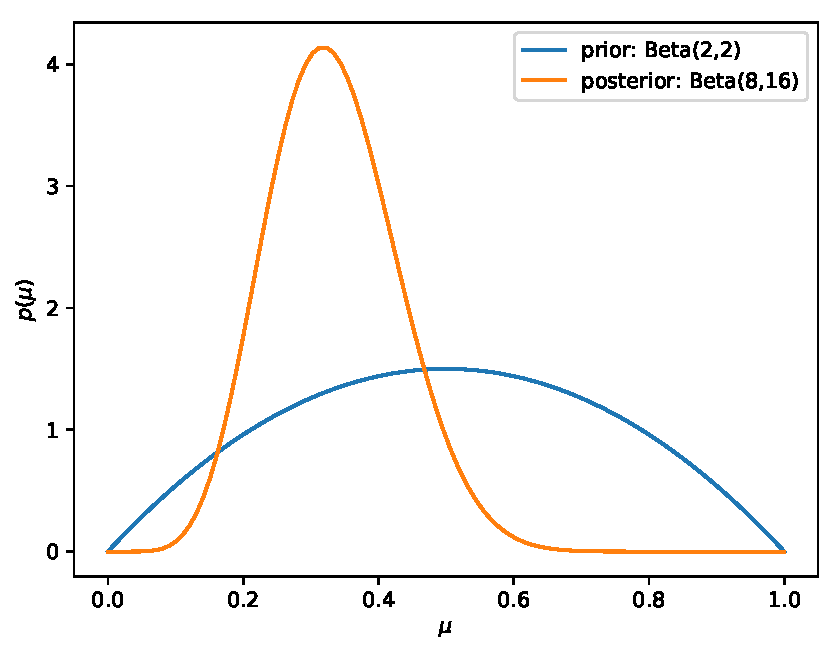
\includegraphics[width = 0.6\hsize]{./figures/beta_distribs.pdf} % this includes the figure and %specifies that it should span 0.7 times the horizontal size of the page
\caption{Pdf and contour plots  for $G_1$ where $\sigma^2_{x_1,x_2} = \sigma^2_{x_2,x_1} = 0$ } % caption of the figure
\label{B1}
\end{figure}

Figure \ref{B1} plots the prior and the posterior, with distributions $\operatorname{Beta(2,2)}$ and $\operatorname{Beta(8,16)}$ respectively.
\pagebreak

\textbf{\begin{itemize}
    \item What has changed from the prior to the posterior? Describe properties of
the prior and the posterior.
\end{itemize}}

As shown in figure \ref{B1}, the shape of the posterior (with $\alpha=8, \beta=16$) is different to the the shape of the prior (with $\alpha=2, \beta=2$). While the prior was symmetric and centered on the [0,1] interval with $mean = median = mode = 0.5$, these properties no longer hold in the posterior. By inspection, the posterior is a narrower distribution and taller distribution.
\bigbreak
For a Beta distribution, it is straightforward to compare the expected value, variance and mode as these all have closed-form solutions. Expected value is:
\begin{align}
    \E[\mu] = \frac{\alpha}{\alpha + \beta}
\end{align}
Computing this, we find the expected value has fallen from $0.5$ to $1/3$. This is expected as the experiment showed a success rate of 30\% so the posterior expected value would be in the interval $(0.3, 0.5)$. We can also compute the variance of a Beta distribution as follows:
\begin{align}
    \operatorname{Var}[\mu] = \frac{\alpha\beta}{(\alpha + \beta)^2(\alpha + \beta + 1)}
\end{align}
We find the variance falls from 0.05 to $1/600=0.0017$. Again, this is expected as we have conducted an experiment on $\mu$ thereby reducing total uncertainty, which is refelcted in a lower variance. We can also compute the mode of the distribution by finding the value $\mu$ which maximizes $p(\mu|x,N,\alpha,\beta) = Beta(8,16)$; i.e. by taking the derivative of the pdf and setting it equal to zero. Doing so yields the following expression for the mode:
\begin{align}
    \operatorname{Mode}[\mu] = \frac{\alpha - 1}{\alpha + \beta - 2}
\end{align}
The mode for the prior is 0.5, and the mode for the posterior is 0.32. As expected, the mode has also fallen. In addition, we see that in the posterior the mode is now less than the mean, so the posterior is positively skewed.
\bigbreak
To summarize, running the experiment has changed the distribution on $\mu$ by reducing the mean, variance and the mode, and has introduced a small positive skew.
\pagebreak





\section{Graphical Models}
\subsection{}
\textbf{[16 marks] Given a factorized joint distribution, draw the corresponding directed graphical model (you can scan in a picture or use the tikz-bayesnet)
\begin{align}
    p(a, b, c, d, e, f) = p(a|b,c)p(c|b)p(d)p(e|d,a)p(f|c,d,e)p(b)
\end{align}}

\begin{figure}[h]
\centering % this centers the figure
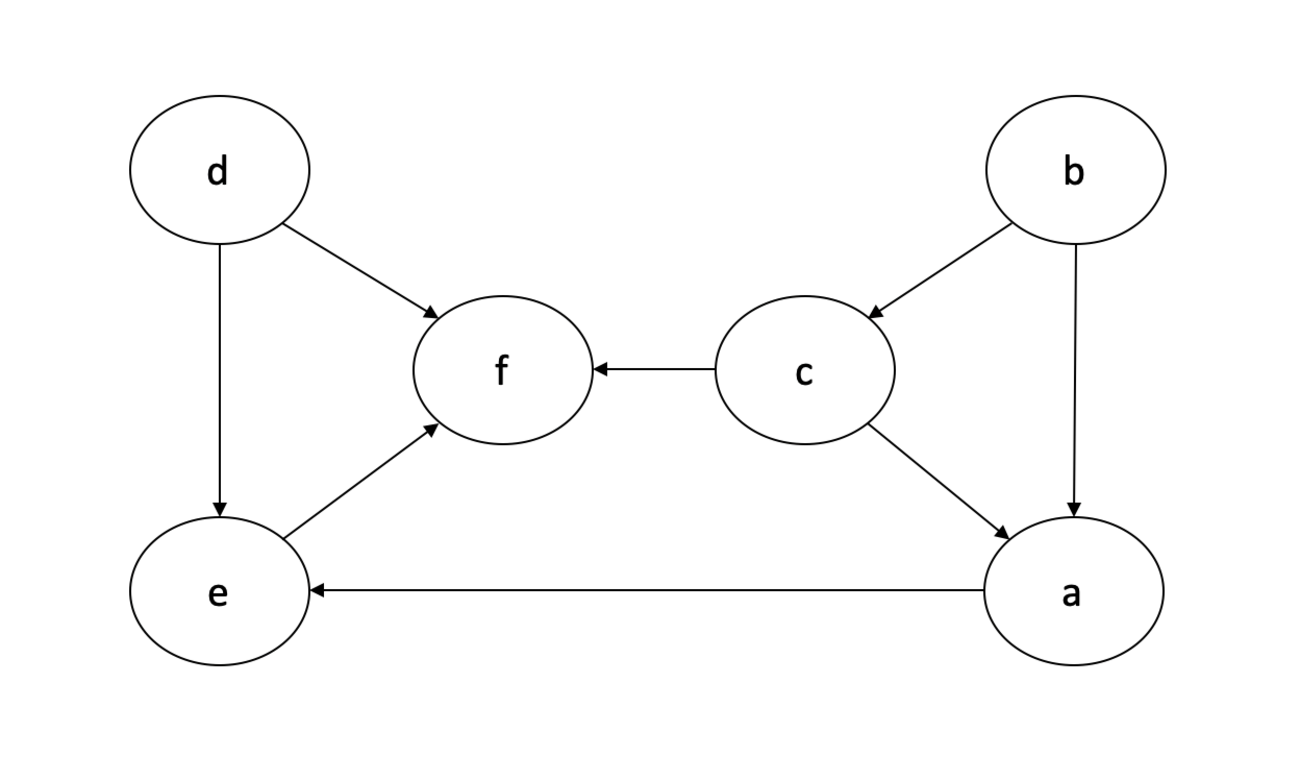
\includegraphics[width = 1\hsize]{./figures/graphical_model.pdf} % this includes the figure and %specifies that it should span 0.7 times the horizontal size of the page
\caption{Graphical model for p(a, b, c, d, e, f) $p(a$} % caption of the figure
\label{GraphicalModel}
\end{figure}



\subsection{}
\textbf{[40 marks] Determine whether the random variables in the graphical are conditionally independent.}
\begin{enumerate}[label=\alph*)]
    \item Conditionally independent: e blocks the path as arrows meet head to head at e and neither e nor its descendants are observed
    \item Not conditionally independent: $h - i - d$; arrows meet head to tail at j and j is unobserved
    \item Conditionally independent: e blocks the path as arrows meet head to head at e (and e's descendants) are unobserved
    \item Not conditionally independent: $j - d - e$; arrows meet head to tail at d and d is unobserved
    \item Not conditionally independent: $b - d - e$; arrows meet head to tail at d and d isn't observed
    \item Not conditionally independent: $j - h - i - c$; arrows meet head to head at h but k is a descendent of h so h is unblocked. arrows meet tail to tail at i and i unobserved so is also unblocked
    \item Not conditionally independent: $a - b - d - k$; all paths are head to tail and no set is observed so none are blocked 
    \item Not conditionally independent: $a - b - d - k$; all paths are head to tail and e is not on the path so path is unblocked
    \item Not conditionally independent: $h - i - d$; arrows tail to tail at i but i isn't observed
    \item Not conditionally independent: $b - j - h$; arrows meet head to head at j but e is a descendant of j so j is unblocked
    \item Not conditionally independent: $h - i - c$; arrows head to tail at i but i isn't observed
    \item Not conditionally independent: $a - b - j - f$; arrows head to tail at b and b isn't observed; arrows are head to head at at j but k is a descendant of j so j is unblocked
    \item Not conditionally independent: $i - h - j - b - a$; h is unblocked as arrows arrive head to head but j is a descendant of h; j is unblocked as arrows are head to head but j is observed; arrows are head to tail at b and b is unobserved to b is unobserved 
    \item Not conditionally independent: $h - j - d - e - g$; arrows are head to tail at j and d and neither are observed so both are unblocked; arrows are head to head at e and e is observed so unblocked
    \item Conditionally independent: e blocks the path (arrows are head to head at e and e is unobserved with no descendants)
    \item Conditionally independent: same as above
    \item Conditionally independent: j and d blocks the paths (j blocks $a - h$ as arrows are head to head at j but j and descendants are unobserved; d blocks $a - i$ as arrows are head to head at d and d and its descendants are unobserved)
    \item Conditionally independent: j and d block paths (j blocks the direct path from $b \rightarrow h$ as arrows are head to head at j and and nothing is observed; d blocks $d - d - i - h$ as arrows are head to head at d but nothing is observed
    \item Conditionally independent: j and d block paths (same reason as question r) as g is not a descendant of j or d)
    \item Conditionally independent: j and d block paths (j blocks $a - b - j - h - i$ as arrows are head to head at j and nothing is observed; d blocks the remaining paths as arrows are head to head at d and nothing is observed)
\end{enumerate}












\end{document}
%%% Local Variables: 
%%% mode: latex
%%% TeX-master: t
%%% End: 
